\section{Test mit allen vorteilhaften Klauseln} % 115 - 80
\label{sec:test_beste}

Nachdem die Klauselmengen in den vorhergehenden Abschnitten einzeln getestet wurden, werden sie in diesem Test gemeinsam genutzt.
Ausgenommen davon sind die Addiererklauseln aus Abschnitt \ref{sec:test_234}, weil sie die Laufzeit negativ beeinflusst haben.
Vernachlässigt wird dabei das negative Ergebnis der Klauseln aus Abschnitt \ref{sec:test_knowledge} in der Variante ohne XOR-Klauseln.
Die resultierende Laufzeit war in diesem Fall nur minimal höher und wird zur besseren Vergleichbarkeit mit der XOR-Variante trotzdem
mit einbezogen. Die Ergebnisse sind in Abbildung \ref{fig:data_final} dargestellt. Wie auch bei den vorhergehenden Tests ist die XOR-Variante
schneller. Die Laufzeit reduziert sich um 20\% gegenüber der Vergleichsbasis, während die Laufzeit der Variante ohne XOR-Klauseln um
15\% ansteigt. Die Anzahl der unterschiedlichen Lösungen hat sich im Bezug zur Vergleichsbasis wenig geändert.
\begin{figure}[!h]
  \centering
  \begin{minipage}[c]{0.45\textwidth}
  \begin{flushleft}Gesamtdauer ohne XOR: 224:36:00\end{flushleft}
  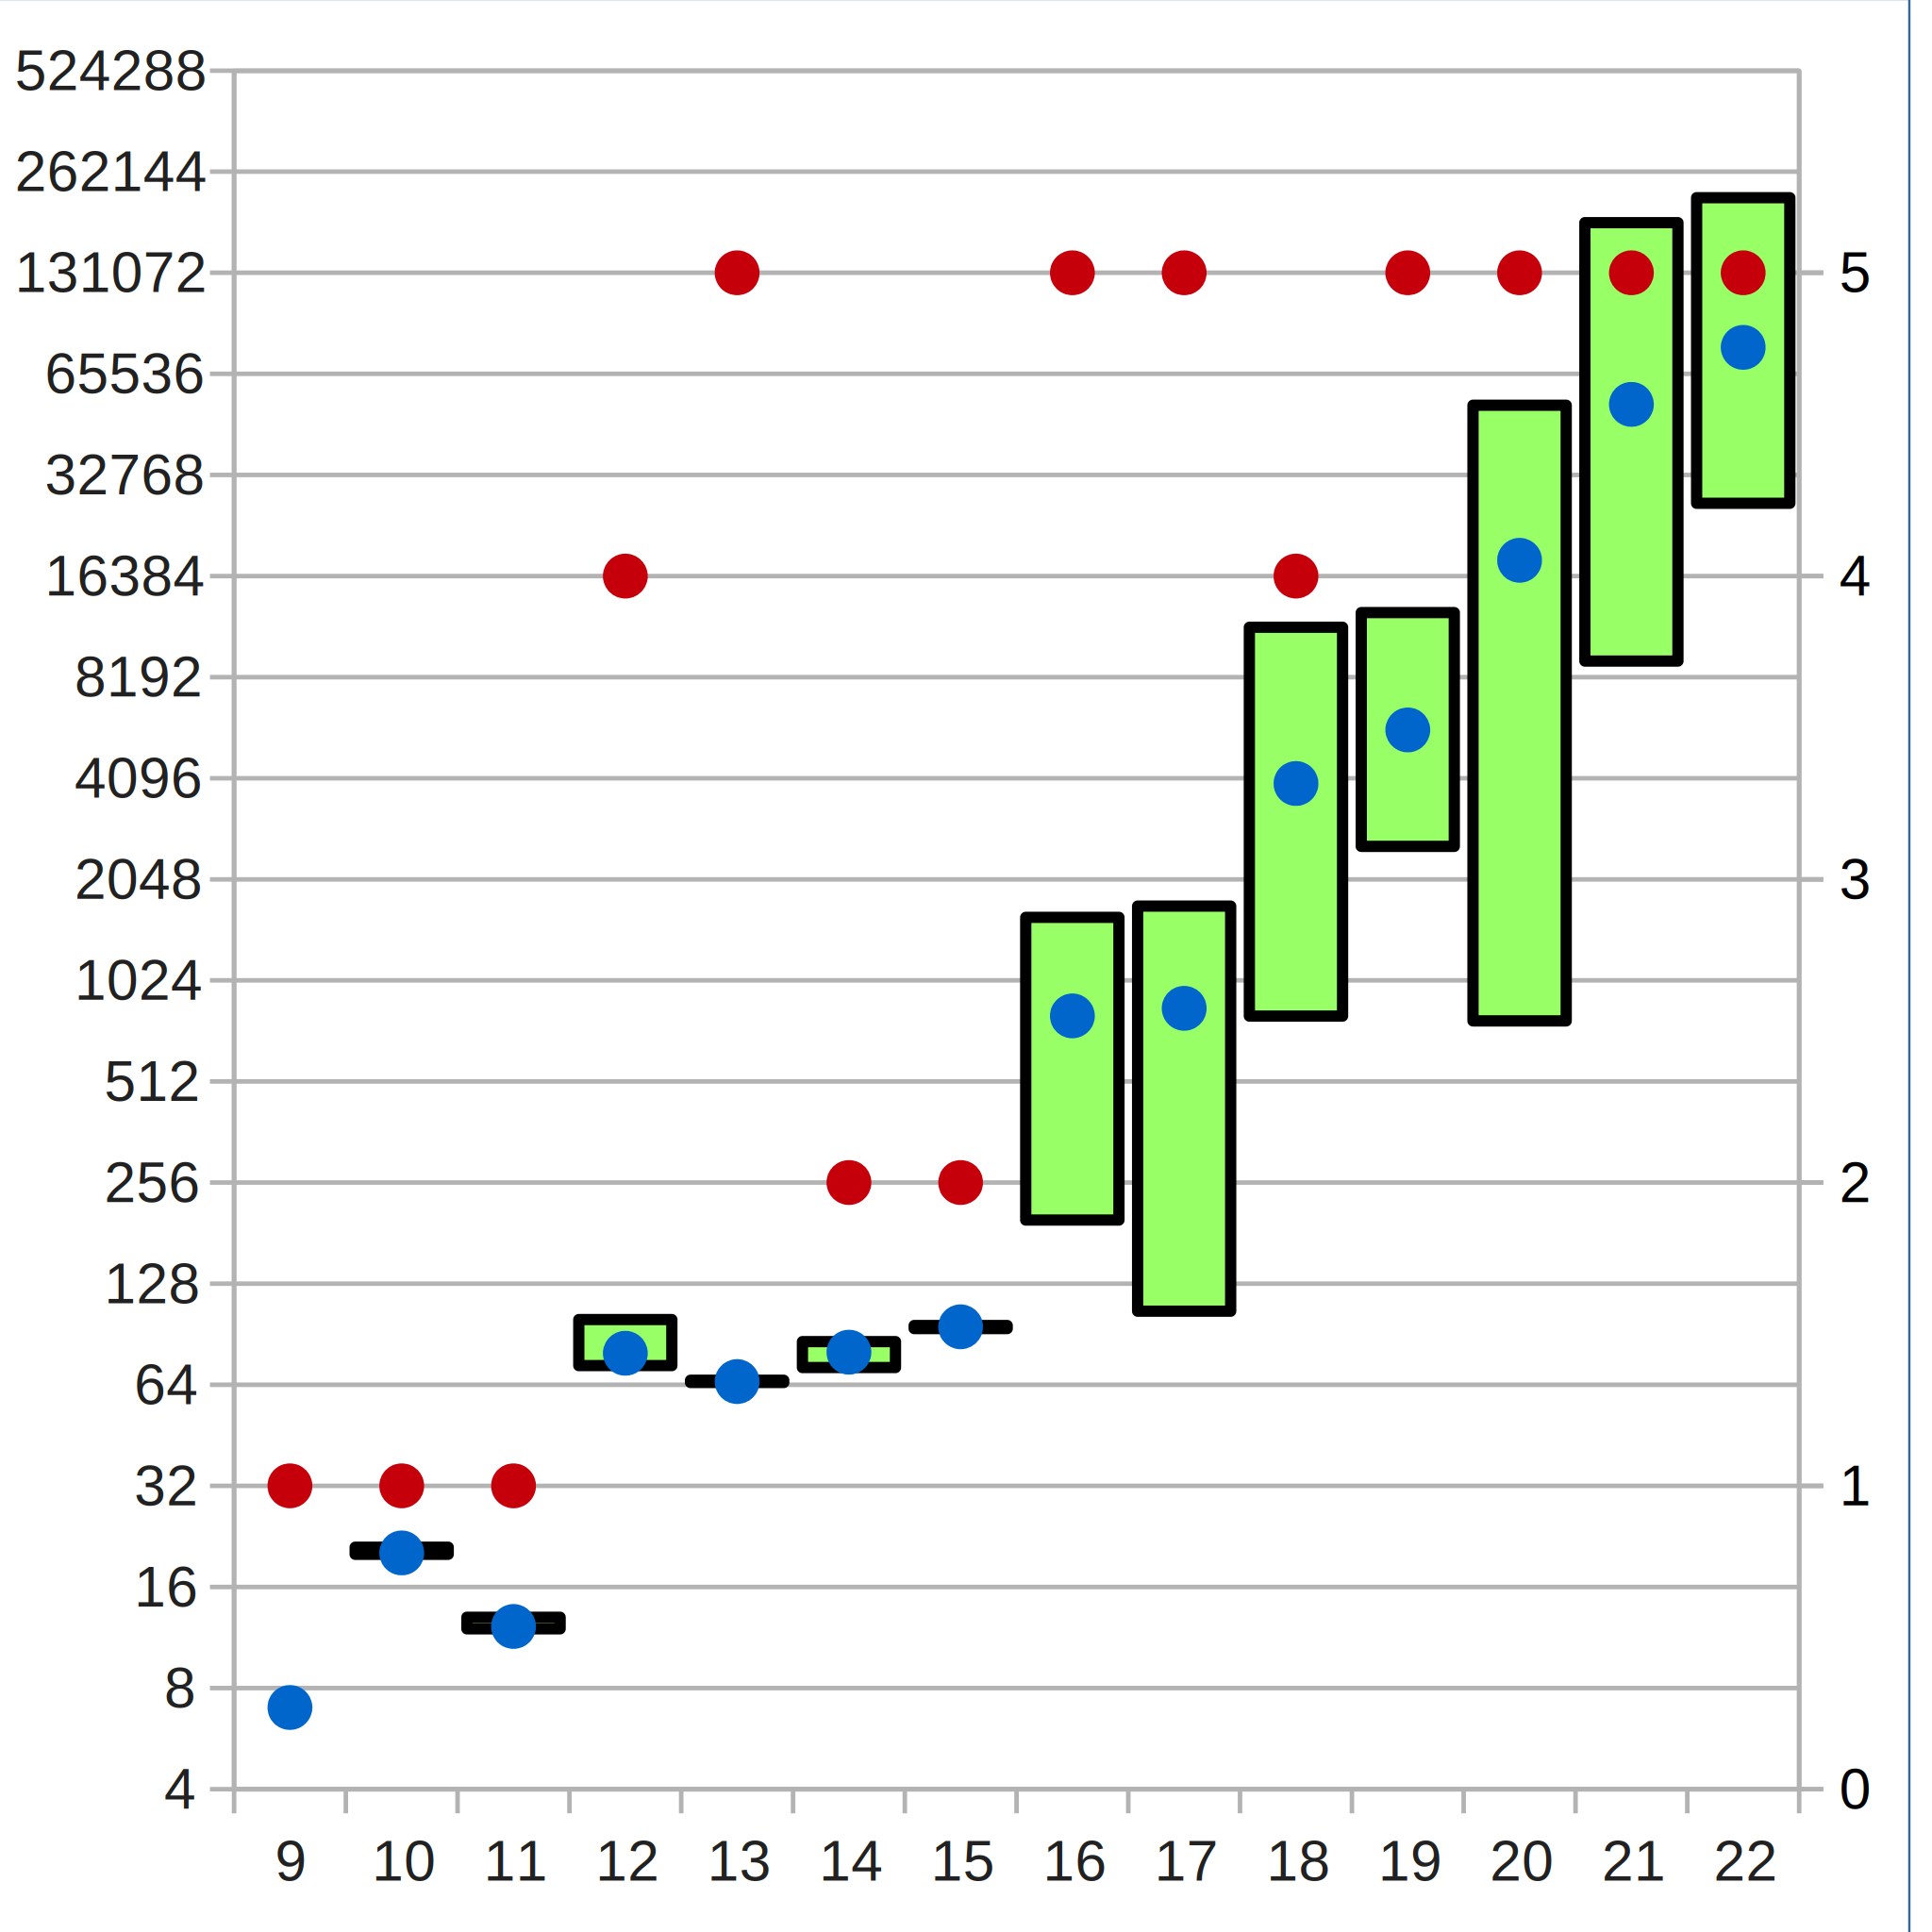
\includegraphics[scale=0.55]{images/data_final_knf}
  \end{minipage}
  \begin{minipage}[c]{0.09\textwidth}
  ~~
  \end{minipage}
  \begin{minipage}[c]{0.45\textwidth}
  \begin{flushleft}Gesamtdauer mit XOR: 136:37:46\end{flushleft}
  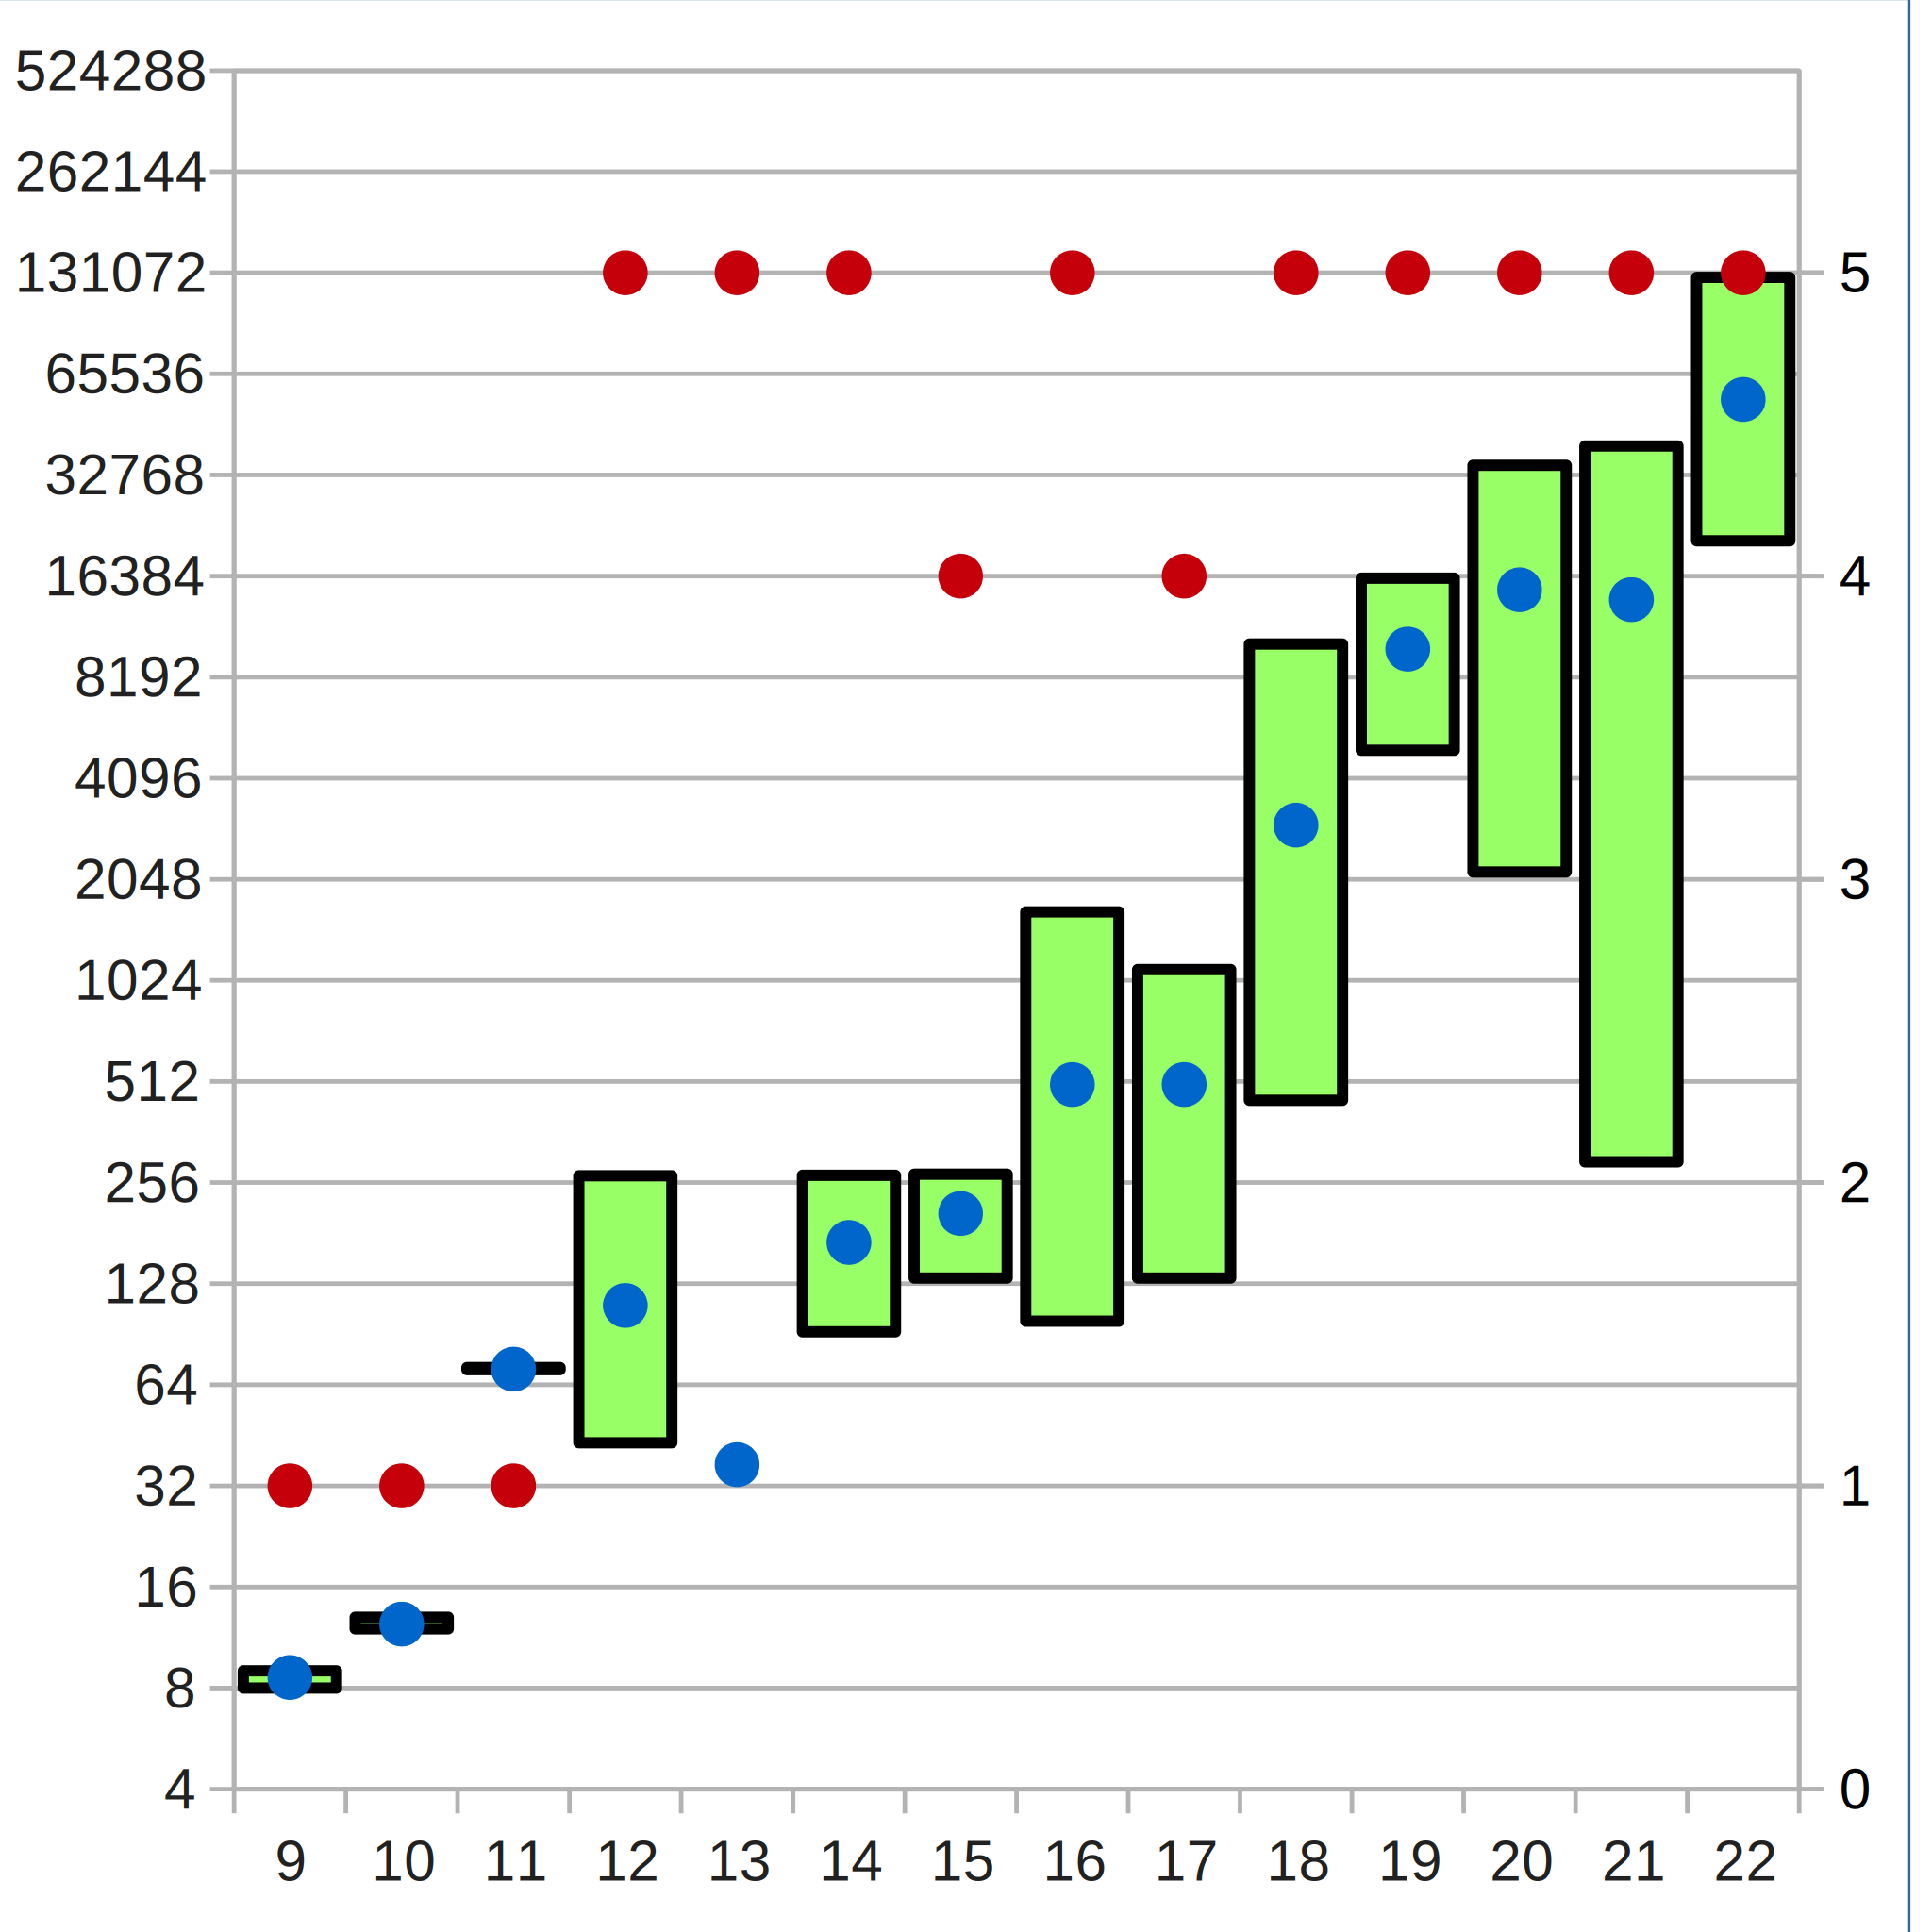
\includegraphics[scale=0.55]{images/data_final_xor}
  \end{minipage}
  \caption{Ergebnisse mit allen vorteilhaften Klauseln}
  \label{fig:data_final}
\end{figure}